\documentclass[a4paper, 12pt]{article}
\usepackage[top=1.8cm, bottom=1.8cm, left=1.5cm, right=1.5cm]{geometry}
\usepackage{amsmath}
\usepackage{listings}
\usepackage{float}
\usepackage{tikz}


\begin{document}
	\begin{center}
		Universidade Federal do Rio Grande do Norte
		
		Departamento de Engenharia da Computação e Automação
		
		DCA3703 - Programação Paralela
		
		\textbf{Tarefa 8 - Coerência de Cache e falso compartilhamento}
		
		\textbf{Aluno:} Daniel Bruno Trindade da Silva
	\end{center}
	
	\section{Introdução}
	\vspace{0.7cm} O número $\pi$ é uma constante matemática fundamental que pode ser estimada através de métodos estocásticos, como a simulação de Monte Carlo. Este trabalho tem como objetivo implementar e comparar diferentes estratégias de paralelização da estimativa de $\pi$ utilizando a biblioteca OpenMP em linguagem C.
	
	Além da implementação, foi feita uma análise do tempo da execução de cada versão, considerando os efeitos da coerência de cache e do falso compartilhamento, fenômenos que impactam o desempenho de aplicações paralelas em arquiteturas modernas.
	
	\section{Metodologia}
	\hspace{.7cm}O método estocástico de Monte Carlo para estimar o valor de $\pi$ é uma técnica probabilística que usa números aleatórios para resolver um problema matemático. Para estimar $\pi$ utilizaremos um circulo de raio 1 circunscrito em um quadrado de lado 2, ambos posicionados no centro do eixo de coordenadas como mostrado na figura 1: 
	
	
	\begin{center}
		\begin{figure}[H]
			\centering
			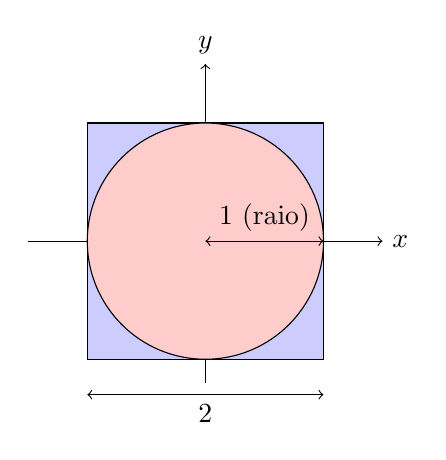
\begin{tikzpicture}[scale=1.5]
				% Eixos coordenados
				\draw[->] (-1.5,0) -- (1.5,0) node[right]{$x$};
				\draw[->] (0,-1.2) -- (0,1.5) node[above]{$y$};
				
				% Quadrado de lado 2 encostado nos eixos
				\draw[fill=blue!20] (-1,-1) rectangle (1,1);
				%\node at (-1,1.2) {Quadrado};
				
				% Círculo de raio 1 à direita do quadrado
				\draw[fill=red!20] (0,0) circle (1);
				%\node at (3,1) {Círculo};
				
				% Marcas de dimensão
				\draw[<->] (-1,-1.3) -- (1,-1.3) node[midway,below]{2};
				%\draw[<->] (0,0) -- (0,1) node[midway,right]{2};
				\draw[<->] (0,0) -- (1,0) node[midway,above]{1 (raio)};
			\end{tikzpicture}
			\caption{Circulo de raio 1 circunscrito em um quadrado de lado 2}
		\end{figure}
	\end{center}
	
	Em seguida geraremos muitos pares (x,y) com valores aleatórios entre 0 e 2, ou seja, dentro da área do quadrado, a proporção de pontos encontrados dentro do círculo em relação ao total gerado se aproxima da razão entre as áreas:
	
	\[
	\frac{\text{Pontos no Círculo}}{\text{Total de Pontos}} \approx \frac{\pi}{4}
	\]
	
	\vspace{1.5cm}
	
	Então para estimarmos o valor de $\pi$ pelo método de Monte Carlo temos:
	
	\[
	\pi \approx 4 \times \frac{\text{Pontos no Círculo}}{\text{Total de Pontos}}
	\]
	
	\vspace{.5cm}
	
	Assim, a base de nosso código será composto por um laço de repetição que gerará \textit{n} pares aleatórios (x,y) e testará se os pontos estão dentro ou não do circulo. Ao final utilizaremos a proporção de acertos pelo número de pares (x, y) para estimarmos o valor de $\pi$.
	
	Nessa tarefa foram desenvolvidos quatro versões do código mudando alguns pontos da abordagem para a paralelização como se segue:
	
	\begin{itemize}
		\item A primeira utiliza a função \texttt{rand()} para geração de números aleatórios, com cada thread acumulando seus acertos em uma variável privada e somando ao total através de uma região crítica \texttt{\#pragma omp critical}.
		
		\item A segunda versão também usa \texttt{rand()}, mas cada thread armazena seus acertos em uma posição distinta de um vetor compartilhado, realizando a acumulação final de forma serial após a região paralela.
		
		\item A terceira e quarta versões seguem a mesma lógica das duas primeiras, porém substituindo rand() por \texttt{rand\_r()}, uma função \textit{thread-safe} que permite melhor paralelização ao eliminar conflitos no gerador de números aleatórios.
	\end{itemize}
	
	Em todas as versões foi utilizada a função \texttt{gettimeofday()} para registrar os tempos de execução e a quantidades de pontos geradas para todas as versões foi de {1.000.000.000}.		
	
	\section{Resultados}
	
	Cada experimento utilizou $10^8$ pontos gerados aleatoriamente e foi executado no mesmo ambiente computacional para garantir a comparação justa.
	
	Os resultados obtidos estão apresentados na Tabela~\ref{tab:resultados}.
	
	\begin{table}[H]
		\centering
		\begin{tabular}{|c|l|c|c|}
			\hline
			\textbf{Versão} & \textbf{Descrição} & \textbf{Tempo (s)} & \textbf{Estimativa de $\pi$} \\
			\hline
			1 & \texttt{rand()} com \texttt{critical} & 13,2701 & 3,141687 \\
			\hline
			2 & \texttt{rand\_r()} com \texttt{critical} & 0,6296 & 3,141577 \\
			\hline
			3 & \texttt{rand()} com vetor compartilhado & 13,9920 & 3,141661 \\
			\hline
			4 & \texttt{rand\_r()} com vetor compartilhado & 0,9164 & 3,141621 \\
			\hline
		\end{tabular}
		\caption{Tempos de execução e estimativas de $\pi$ para cada versão do código.}
		\label{tab:resultados}
	\end{table}
	
	Observa-se que todas as versões forneceram estimativas bastante próximas do valor real de $\pi$ (aproximadamente 3,14159265), com diferenças esperadas para um método estocástico baseado em amostragem aleatória.
	
	Quanto ao desempenho, foi possível observar que:
	
	\begin{itemize}
		\item As versões que utilizam \texttt{rand\_r()} apresentaram tempos de execução significativamente menores, devido à natureza \textit{thread-safe} desta função, que evita conflitos no acesso ao gerador de números aleatórios.
		\item A eliminação da região crítica através do uso de um vetor compartilhado melhorou o desempenho, porém o uso da função \texttt{rand()} ainda limitou a velocidade nas versões correspondentes.
		\item Mesmo nas versões vetorizadas, o falso compartilhamento pode ter impactado levemente o desempenho, pois múltiplas threads escrevem em posições adjacentes de memória, afetando a eficiência da cache.
	\end{itemize}
	
	\section{Análise dos Resultados}
	
	A análise dos resultados obtidos permite identificar diferentes fatores que influenciam o desempenho das versões paralelas da estimativa estocástica de $\pi$. Dois aspectos principais devem ser destacados: o impacto da função geradora de números aleatórios utilizada (\texttt{rand()} versus \texttt{rand\_r()}) e a organização do acesso à memória compartilhada pelas threads.
	
	\subsection{Impacto da função geradora de números aleatórios}
	
	As versões que utilizam \texttt{rand\_r()} apresentaram tempos de execução significativamente menores em comparação às versões que utilizam \texttt{rand()}. Isso ocorre porque \texttt{rand()} é uma função tradicionalmente \textit{não thread-safe}, ou seja, seu uso simultâneo por múltiplas threads gera contenção em torno de variáveis internas globais, introduzindo atrasos devido à necessidade de sincronização implícita.
	
	Já \texttt{rand\_r()} é uma função \textit{thread-safe} que opera sobre uma semente local passada por argumento. Cada thread pode, portanto, gerar seus próprios números aleatórios de forma independente, sem interferência entre si. Essa independência elimina a contenção no gerador de números aleatórios e permite que as threads realmente executem em paralelo, maximizando o ganho de desempenho com o uso de múltiplos núcleos.
	
	\subsection{Impacto da estratégia de acumulação e falso compartilhamento}
	
	Outra diferença entre as implementações está relacionada à forma como as threads acumulam os acertos:
	
	\begin{itemize}
		\item Nas versões com \texttt{critical}, cada thread utiliza uma variável local para contar seus acertos, mas a atualização da variável global de hits ocorre dentro de uma região crítica. Como apenas uma thread pode executar dentro da região crítica por vez, existe uma limitação na escalabilidade do desempenho, especialmente conforme o número de threads aumenta.
		
		\item Nas versões vetorizadas, cada thread escreve seus acertos em uma posição exclusiva de um vetor compartilhado. Isso elimina a necessidade de regiões críticas durante a execução principal, favorecendo a paralelização e melhorando o desempenho geral.
	\end{itemize}
	
	No entanto, o uso de vetores compartilhados pode introduzir um outro fenômeno conhecido como \textbf{falso compartilhamento} (\textit{false sharing}). O falso compartilhamento ocorre quando múltiplas threads acessam e modificam variáveis que estão armazenadas em posições de memória próximas e que pertencem à mesma linha de cache. Mesmo que cada thread acesse apenas sua própria posição do vetor, a arquitetura do sistema pode fazer com que modificações próximas invalidem linhas de cache, resultando em atualizações frequentes e ineficientes entre os caches dos processadores.
	
	O falso compartilhamento gera penalidades de desempenho, pois aumenta a comunicação e a sincronização implícita entre os núcleos, reduzindo o ganho esperado de paralelismo.
	
	Apesar disso, nos resultados obtidos, o impacto do falso compartilhamento foi relativamente pequeno em comparação ao ganho expressivo obtido pela eliminação da região crítica e pela adoção da função \texttt{rand\_r()}.
	
	\section{Conclusão}
	
	Neste trabalho, foi realizada a implementação e análise de quatro versões paralelas para a estimativa de $\pi$ utilizando o método de Monte Carlo com OpenMP.
	
	Observou-se que o uso da função \texttt{rand\_r()}, por ser \textit{thread-safe}, proporcionou ganhos significativos de desempenho em relação à função \texttt{rand()}, eliminando a contenção entre as threads. Além disso, a substituição de regiões críticas por vetores compartilhados também melhorou a eficiência, apesar do leve impacto do falso compartilhamento.
	
	Conclui-se que, para otimizar aplicações paralelas, é essencial adotar geradores de números aleatórios adequados ao ambiente multi-thread e estruturar o acesso à memória de forma a minimizar conflitos de cache.
	
	
\end{document}